%%%%%%%%%%%%%%%%%%%%%%%%%%%%%%%%%%%%%%%%%%%%%%%%%%%%%%%%%%%%%%%%%%%%%%%%%%%%%%%%%%%%%%%%%%%%%%%%%%%%%%%

\documentclass[prb,aps,12pt,superscriptaddress,floatfix]{revtex4-2} 
\usepackage{graphicx}
\usepackage{color} 
\usepackage{amsmath}
\usepackage{amssymb} 
\usepackage{natmove}
\usepackage{natbib}
\usepackage{hyperref} 
\usepackage{bm}

%%%%%%%%%%%%%%%%%%%%%%%%%%%%%%%%%%%%%%%%%%%%%%%%%%%%%%%%%%%%%%%%%%%%%%%%%%%%%%%%%%%%%%%%%%%%%%%%%%%%%%%

\begin{document}

\title{\huge On the Origin of Shrimpoluminescence}

\author{\large Tyler C. Sterling}
\email{ty.sterling@colorado.edu}
%\affiliation{Department of Physics, University of Colorado at Boulder, Boulder, Colorado 80309, USA}

\date{\today}

%\begin{abstract}
%\end{abstract}

\maketitle

%\listoffigures
%\listoftables
%\tableofcontents

%%%%%%%%%%%%%%%%%%%%%%%%%%%%%%%%%%%%%%%%%%%%%%%%%%%%%%%%%%%%%%%%%%%%%%%%%%%%%%%%%%%%%%%%%%%%%%%%%%%%%%%

\begin{figure}
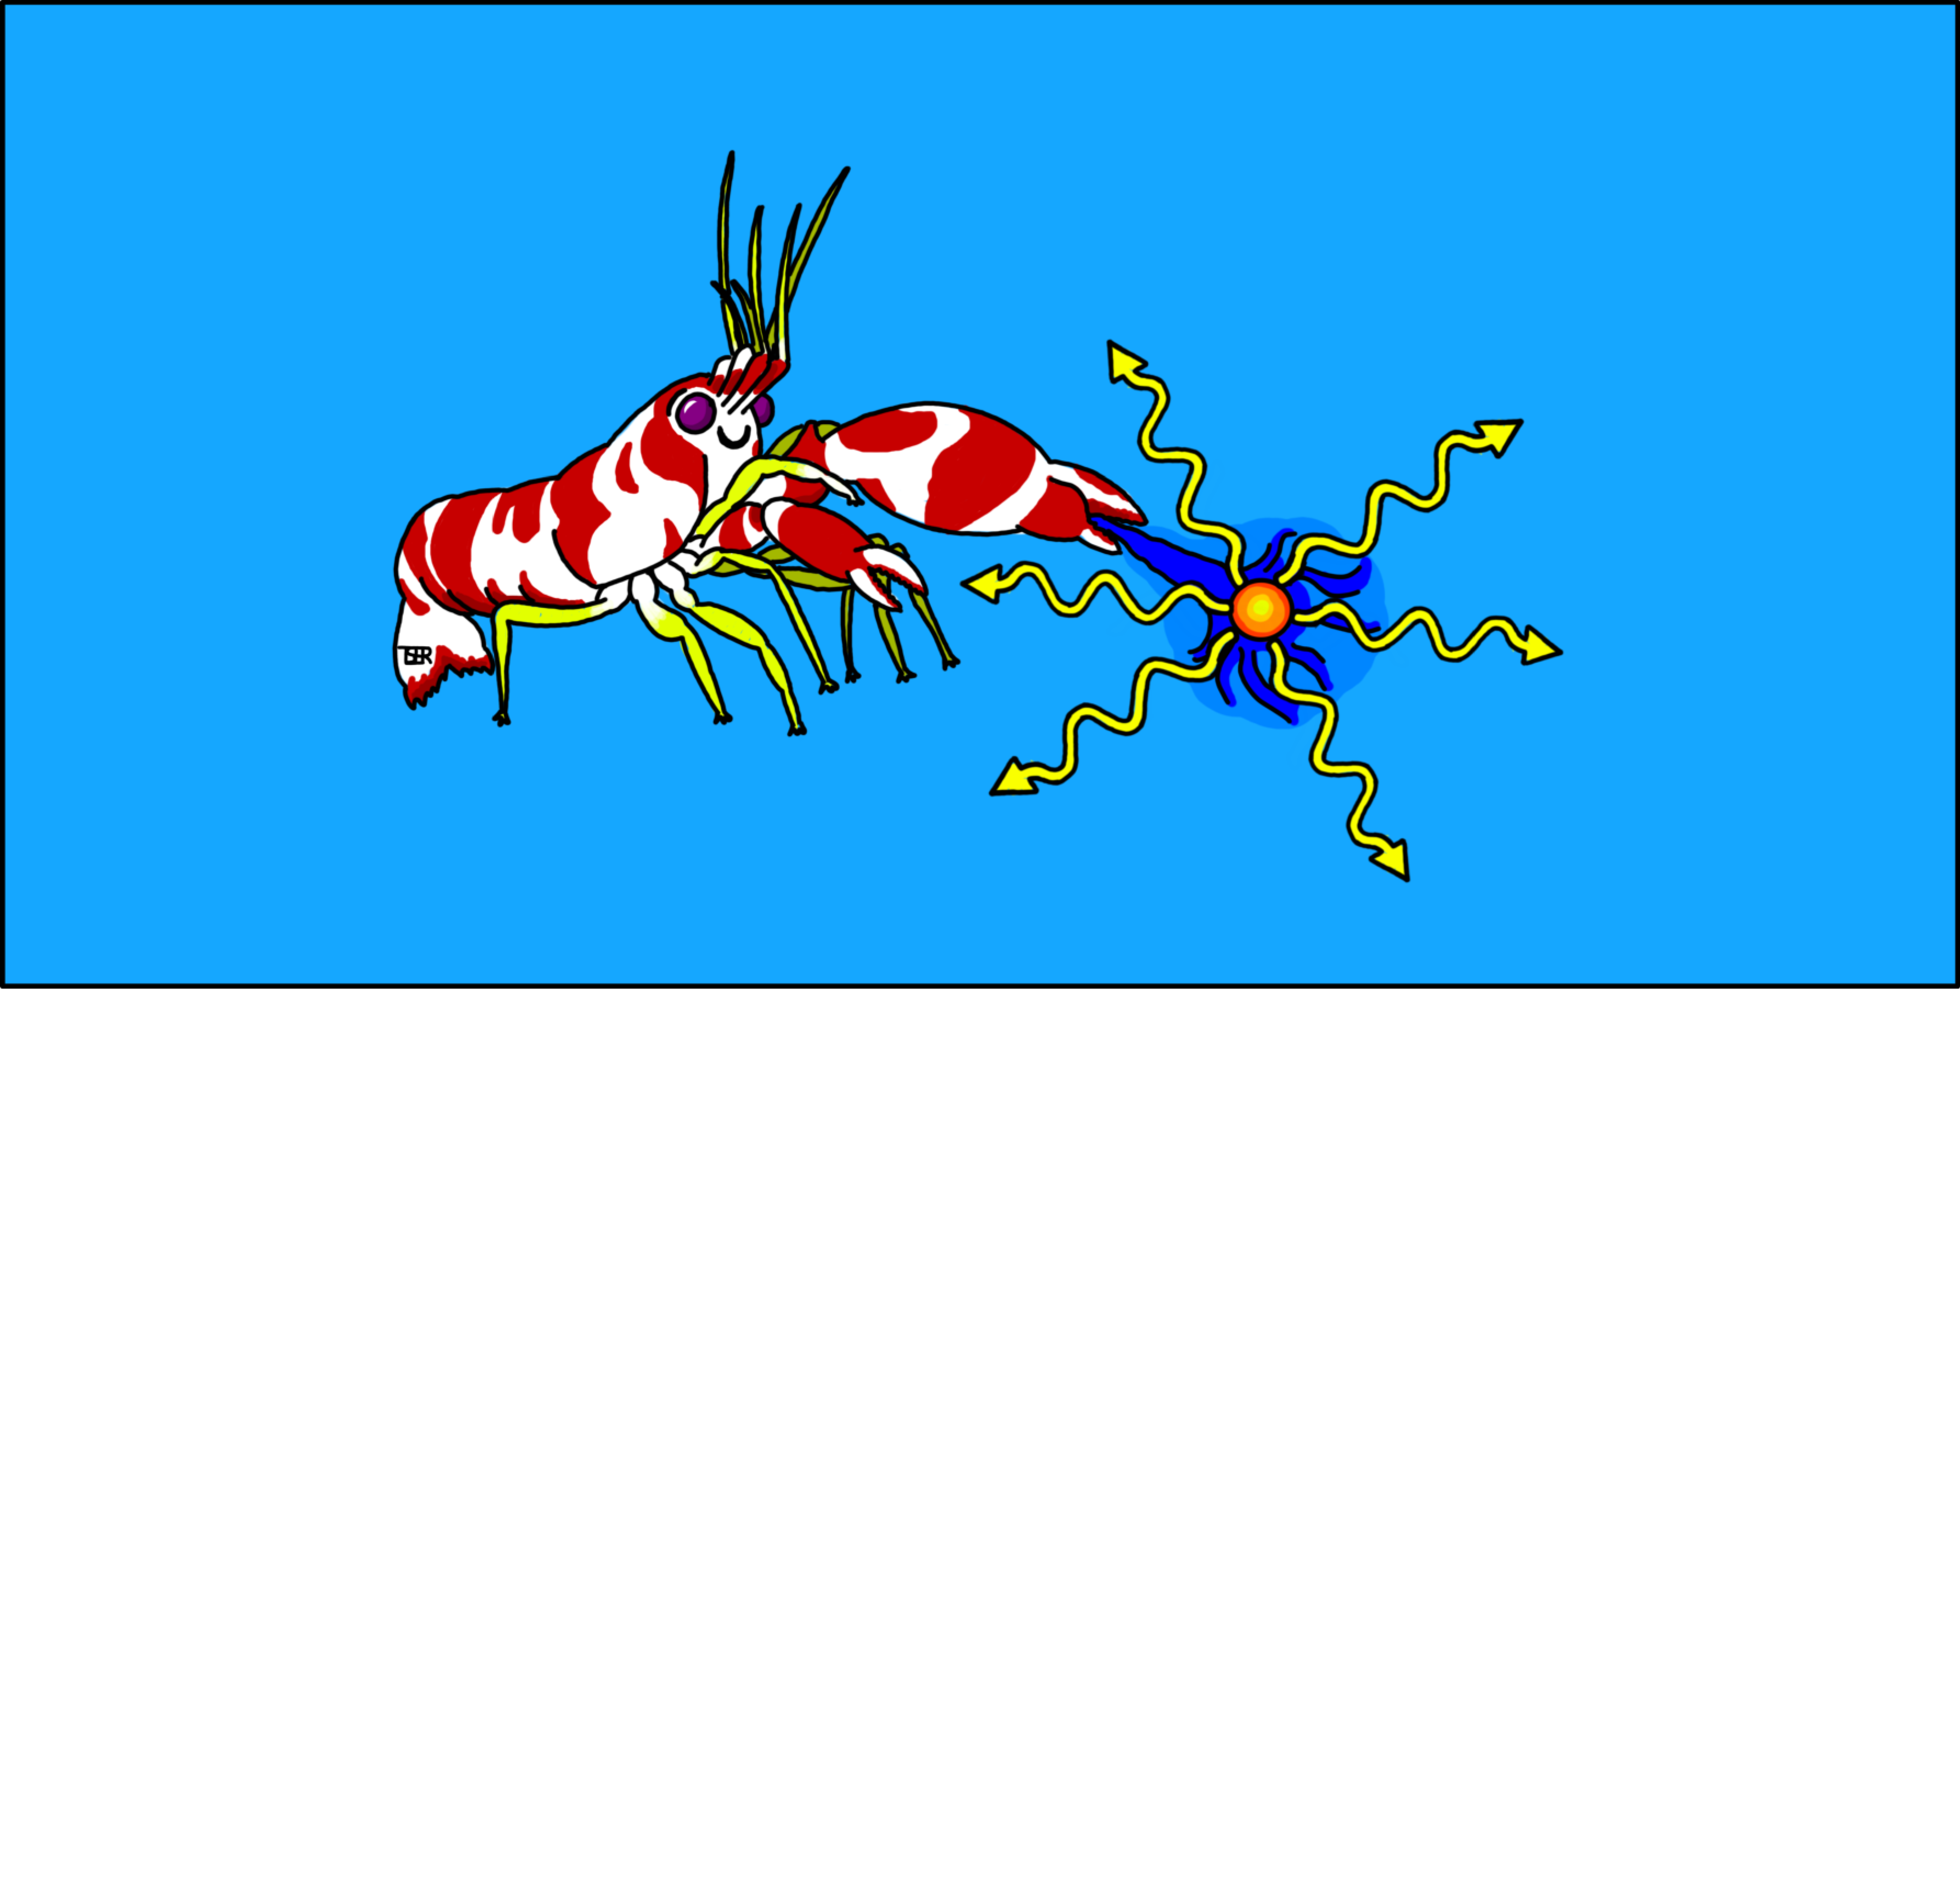
\includegraphics[width=1\linewidth]{../figs/shrimpy2.pdf}
%    \caption{}
\label{fig:shrimpy}
\end{figure}

 
\newpage

\section{QED}
the ref \cite{liberati2000sonoluminescence} has lots of good refs. they have follow up papers extending Schwingers papers (which are refd therein) and referencing a bunch of other relevant literature. I should look for refs citing Schwingers paper to try to figure out the modern state of the art of this thin.

\section{Modelling}
in the ref \cite{schanz2012molecular}, they use MD to modelling the equation of state for a collapsing bubble. they calculate the temperature and study the conditions for emitting light.

\section{Refs. to different arguments}
ref \cite{didenko2000molecular} gives examples of other origin theories (molecular excited states, black-body radiation, bremsstrahlung, ion-electron recombination, confined electrons)


%%%%%%%%%%%%%%%%%%%%%%%%%%%%%%%%%%%%%%%%%%%%%%%%%%%%%%%%%%%%%%%%%%%%%%%%%%%%%%%%%%%%%%%%%%%%%%%%%%%%%%%

\bibliography{../ref}

\end{document}
